% !TeX encoding = utf8
% !TeX root = ./main.tex

% part I
% \titleformat{\chapter}
%   {\chap}{\thechapter}{1em}{}
% \titlespacing*{\chapter}{0pt}{3.5ex plus 1ex minus .2ex}{2.3ex plus .2ex}
%
\part{毕业论文}

% -------------------------------------------------------------------------
\chapter{引言}
% -------------------------------------------------------------------------

\section{研究背景与意义}

近年来,随着城市安防越来越被重视,安防监控系统越来越普及。
复杂的摄像头网络和海量的视频数据,使得依赖人力观察每个监控设备视频的方法不再适用。
智能行人监控技术应运而生,其中行人再识别(Person Re-identification, Person Re-ID)作为智能行人监控系统的核心技术之一,成为一个新的研究热点。
近几年,行人再识别领域投稿数量和性能均大幅增长,
2015年性能指标CMC-1(Cumulative Matching Characteristic with Rank-1, 只考虑第一个预测结果的累计匹配因子)
只有$65\%$。17年达到了$80\%-85\%$。随后17年11月,在Arxiv上抢先公布的技术报告已经达到了$90\%-96\%$,号称在大型数据集上超越人类的表现。预计18年行人再识别领域会有更多应用和突破。

图~\ref{fig:overall}为广义的行人再识别过程。
广义的行人再识别可以被分解为三个步骤:行人检测(Pedestrian Detection),
行人跟踪(Pedestrian Tracking),
行人检索(Pedestrian Retrieval)。
其中行人检测是从视频监控视频每一帧中检测出行人的技术;
行人跟踪是在时序上将行人串联起来形成视频片段的技术;
而行人检索是利用得到的行人图像完成跨摄像头行人检索的技术。
根据Zheng \etal \cite{zheng2017person}的定义,行人检测和行人跟踪是计算机视觉中已经存在的任务,因此大多研究者所指的狭义的行人再识别问题(Person Re-identification,Person Re-ID)着力解决第三个模块,也即
行人检索问题。
本文也不例外,着力解决狭义的行人再识别问题,也即行人检索问题。

\begin{figure}
	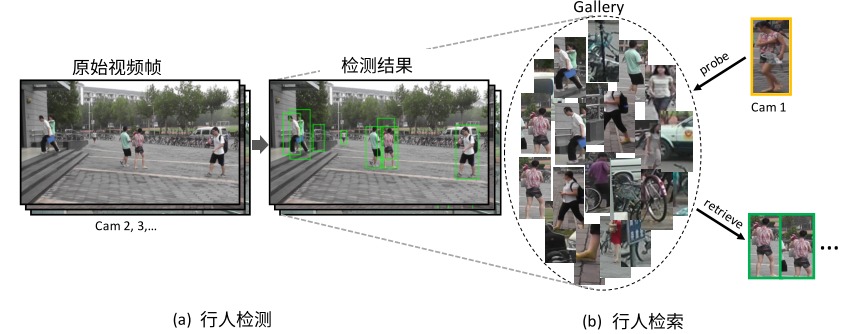
\includegraphics[width=\textwidth]{background.png}
	\caption{广义的行人再识别任务的总体框架,图片修改自~\cite{zheng2017person}}
	\label{fig:overall}
\end{figure}

\section{国内外研究现状}

目前国内外行人再识别的研究主要集中在两方面的关键技术:提取具有鉴别力的行人特征和度量匹配空间的学习。

首先是提取具有鉴别力的行人特征。
具有鉴别力的行人特征必须能够反映行人最基本的区别于其他行人的特征,
同时需要对
环境的变化和行人本身的变化具有一定的鲁棒性,
包括明暗变化、环境噪声和行人姿态变化等;
现有的工作通常融合全局特征和局部特征\cite{reciprocal},\cite{liu2017hydraplus},\cite{zhao2017spindle},\cite{glad},或引入注意力机制。
比如,Li \etal \cite{latent}使用STN结合先验定位可变性的行人部分,
从原始图片中预测定位参数,便于后续的网络将注意力集中于具有潜在语义的身体部分。
考虑到视频监控环境下行人的姿态先验——行人通常直立于地面,作者使用了4个自由度的仿射变换矩阵,建模了尺度、平移方面的可变性变换。
最终提取出更具有鉴别力的行人特征。

其次是度量匹配空间的学习,
对于行人再识别任务,
我们需要定义在原始像素空间和最终特征空间的距离度量函数,
使得具有相同身份的行人图像距离尽可能小,一致性度量标准尽可能大,
同时最大化不同身份的行人图像距离,最小化一致性度量标准。
行人再识别的实际输入通常是一些从未在训练集中出现过的行人图片,从中提取特征,继而进行相似性度量或距离度量。由于这样的特性,分类问题学习每个类别模板来区分不同类别的方法不再适用。 
尽管ImageNet时代大规模分类任务\cite{deng2009imagenet}
取得了惊人的效果,
但是不可能学习所有行人的模板,
即使有充足的数据、学习了尽可能多的行人的模板
分类方法也只能保证已知类别行人图片的可分性,
对此,国内外学者提出了大量
度量学习损失函数,包括对比损失(Contrastive loss)\cite{varior2016gated}、三元组损失(Triplet loss)\cite{schroff2015facenet}、四元组损失(Quadruplet loss)\cite{chen2017beyond}、难样本采样三元组损失(Triplet hard loss with batch hard mining, TriHard loss)\cite{hermans2017defense}、边界挖掘损失(Margin sample mining loss, MSML)\cite{xiao2017margin}。希望通过直接学习欧式空间中的嵌入特征,并使用欧氏距离度量,完成再识别任务。

\section{主要研究内容}

我们使用深度网络提取有鉴别能力的行人特征,
目标是应对各种可能的复杂环境,
包括
相机参数的差异、视角的变化,
行人的非刚性姿态变换,
行人穿着、尺度的变化,
环境的明暗、遮挡等。

面对上述诸多挑战,虽然已经有很多前人的研究成果,比如Guo \etal\cite{guo2018multilevel}和Chang \etal\cite{chang2018factor}通过层次化的方法提取有鉴别能力的行人特征,但是仍然有很多值的考虑地方:

\begin{itemize}
	\item \cite{zhao2017part} 在得到全局的特征之前的同一阶段同时提取局部特征,是否存在信息的冗余?
	      不同的局部特征,比如背包、头发,应该如何与全局特征融合,是使用训练结束就固定的权重,还是使用与输入有关的动态权重?
	      % discard?or put to future work?
	\item 对于存在空间失配的再识别问题,采用什么样的注意力机制最为合适?我们观察到\cite{zhao2017part} 每增加一个分支,就会增加许多参数和计算量,如何在引入注意力机制的同时,权衡复杂度与性能之间利弊?
\end{itemize}

在度量学习方面,我们首先在真实数据集上可视化了现有损失函数,分析了各个损失的优缺点。
总结起来,\textbf{(1)、}中心损失对各个类别给以相同的重视程度,但是不同类别之间容易被混淆的程度是不一样的。
同时中心损失本身只考虑类内距离,因此单独使用无法做到类间散度最大化;
\textbf{(2)、}
如前所述,交叉熵损失基于线性最优分类器的想法,只能在封闭环境下。它学得的决策分界面具有可分性,但不具有鉴别性;
\textbf{(3)、}
基于实例的度量损失,如二元组或三元组损失,如果没有在线难样本挖掘的帮助\cite{yaqing2016semantics},仅仅依靠随机选择样本对和更长的训练时间,会导致模型过度强掉简单样本,进而导致性能下降。
\textbf{(4)、}
基于实例的度量损失,如三元组损失,在难样本挖掘的帮助下,能找到最富有信息的样本,并利用这些代表性的样本实现类间间距最大化。
但是即使考虑了不同类别之间最大化边界,
在实验中我们观察到,这种损失泛化到测试集时仍然可能因为某些类别的散度较大,
存在一些样本偏离到边界,容易和开放环境下的其他样本或潜在的类中心混淆。

随后我们提出了对比中心损失,联合三元组损失共同监督,端到端地学习了使用深度网络作为核函数的度量函数,
有效提升了行人再识别的CMC-1和mAP指标。

% -------------------------------------------------------------------------
\chapter{基于注意力机制的多尺度特征融合}
% -------------------------------------------------------------------------

\section{问题概述}

行人再识别旨在学习鲁棒的特征,达到最小化类内间距和最大化类间间距的目标。
但是由于跨摄像头检索时,环境和行人姿态的各种变化,导致模型很难自发地学到具有鉴别能力的特征。
同时,由于检测器的误差,导致行人图片存在一定的空间维度偏移,即空间失配,给行人再识别带来了极大的挑战。
如图~\ref{fig:label2det}所示,我们在CUHK03人工标注数据集和CUHK03检测其自动检测数据集上,训练了相同的基准模型,
在CUHK03人工标注版本的数据集上,基准模型预测结果与期望结果完全一致;而在CUHK03检测器自动检测的数据集上,
由于测试集中的图片存在严重的空间失配,五个预测结果没有一个正确。
其中模型认为最为可能的预测结果,由于受到了询问图片中红色背景的干扰,从候选集中挑选了一张存在红色遮挡物的图片。可见,模型应当将注意力集中于前景区域,从而提取鲁棒的行人特征。对此,我们提出了基于注意力机制的多尺度特征融合方法。其中多尺度机制有助于高分辨率的局部特征在没有信息损失的情况下参与到最终的行人特征表示;注意力机制有助于去除中层属性特征的背景干扰。

\begin{figure}
	\centering
	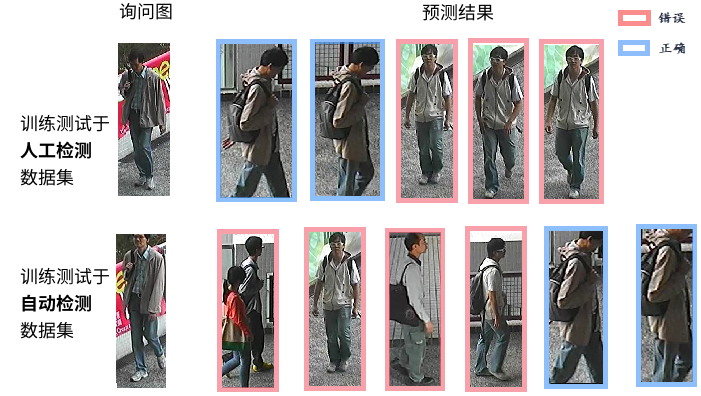
\includegraphics[width=.95\textwidth]{2018-04-18-21-53-15.png}
	\caption{我们的基准模型在手工标注的数据集和行人检测器自动检测的数据集上的典型样例} \label{fig:label2det}
\end{figure}

传统的工作中通常直接使用深度神经网络的最后一层定义统一的特征空间。
但是想要应对各种变化,中层的局部特征也非常重要\cite{yu2017devil},
于是,我们 
通过注意力机制,抽取、凝练中层属性特征中的重要信息,然后与高层语义特征融合。
我们提出的模型在网络结构上引入先验,从而融合高层语义特征和中层属性特征。
模型包含两个模块:\textbf{(1)、}基于注意力机制的多尺度属性特征提取模块;\textbf{(2)、}特征融合与度量学习模块。

\section{框架设计及算法实现}

\subsection{多尺度属性特征提取模块}

基础的骨架网络采用卷积神经网络结构。可以采用的结构包括残差神经网络(ResNet)\cite{he2016identity}、Inception网络\cite{szegedy2015going}以及Squeeze \& Extraction网络\cite{hu2017senet}等。

为了说明我们方法的有效性,我们采用在ImageNet上预训练好的ResNet-50模型,这是目前最为通用的基础骨架模型。
该模型采用全卷积的架构,即所有的参数层都可用卷积层实现。
一般的方法直接对最后一层卷积层的特征进行全局池化,获得图像的表示$x_4$。
由于在环境、姿态、视角的变化,使用全局特征往往不能很好地鉴别不同的行人,所以
我们同时使用中间层特征来补充$x_4$。
这样的策略,从前向传播的角度看,保证了最终的表示有效包含高分辨率的中层属性信息;从反向传播的角度看,保证了监督信息有效反传更新中层特征,有助于学到更加有鉴别力的表示。

考虑到行人再识别中,姿态的多变、相机视角的差异都会导致严重的空间失配,图像的空间信息不是很可靠,
简单地池化拼接中层属性特征反而会引入背景噪声,造成性能下降,
这一点我们在CUHK03检测数据集上得到了验证。
于是我们引入了在通道层面压缩抽取的注意力机制。
之所以引入通道层面的注意力机制,而不是空间上的注意力机制,是基于以下观察:
\textbf{(1)、}目前主流的分类网络,包括残差网络,都在最后一层采用全局池化,抛弃空间信息。这样的做法导致预训练好的模型倾向于将行人的不同高层语义部件或中层属性特征分布在通道层面,而不是混合在同一通道中。
\textbf{(2)、}可视化深度网络高层的特征图可以发现,它的同一通道的激活值往往具有稀疏性,这种稀疏性不是传统意义上的有很多接近于零的激活值,而是同一个通道内的激活值往往表示同一个概念或者行人部件。因此与其再使用空间层面的注意力,倒不如相信深度网络本身已经实现了在同一通道内集中注意力于一个概念。于是更重要的是对不同的语义部件或属性特征进行有选择性地强调、甚至创造新的语义部件或属性特征来替换不重要的。
参考Hu \etal \cite{hu2017senet},我们采用在通道层面压缩和激活的注意力机制。这样的方法在ImageNet分类任务上效果获得了较好的效果。
一方面,这种方法能够避免空间信息的噪声干扰,使得最终的特征更为鲁棒;
另一方面,这种方法基本不增加计算量和显存开销。

\begin{figure}
	\centering
	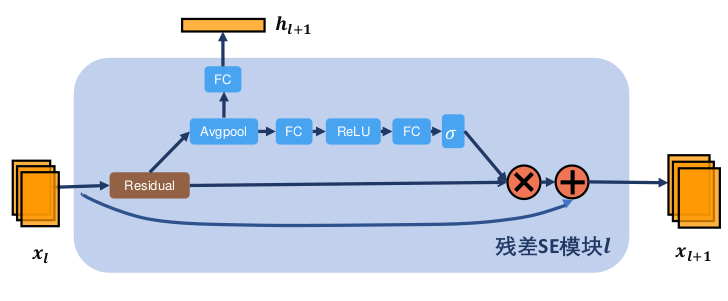
\includegraphics[width=.9\textwidth]{fig/2018-05-11-16-53-10.png}
	\caption{兼具提取属性特征作用的残差SE模块}
	\label{fig:resse}
\end{figure}

如图~\ref{fig:resse}所示,我们基于\cite{hu2017senet}提出了残差SE模块,用于替换残差网络中的瓶颈模块(Bottleneck Block)。
该模块通过通道级别特征响应的重新组合,自动选择出具有鉴别力的特征或重新组合创造出新的特征,从而将有限的计算资源分配于计算最富有信息量的特征信号分量。
% 公式也许
从计算量的角度看,由于浅层属性特征的通道维度通常较小,增加通道级别的注意力重组机制不需要耗费过多的计算量;
但是高层语义特征的通道维度通常较高,会增加计算量和参数,增加过拟合的风险。
但是幸运的是,通过实验,Hu \etal 发现最终的全局特征
不需要进一步使用通道层面的注意力机制。
因为即使使用了注意力机制,
,学习到的注意力权重也接近于均匀分布。
这说明,最终的全局表示在每一个通道上都有特定的语义信息,冗余程度较小,重要程度相同。
遵循这一观察,我们进一步提出在特征融合阶段自适应地重用每个阶段抽取的属性特征$h_{l+1}$。

% \misscite Resource Aware Person Re-identification across Multiple Resolutions
% \begin{figure}
% 	\centering 
% 	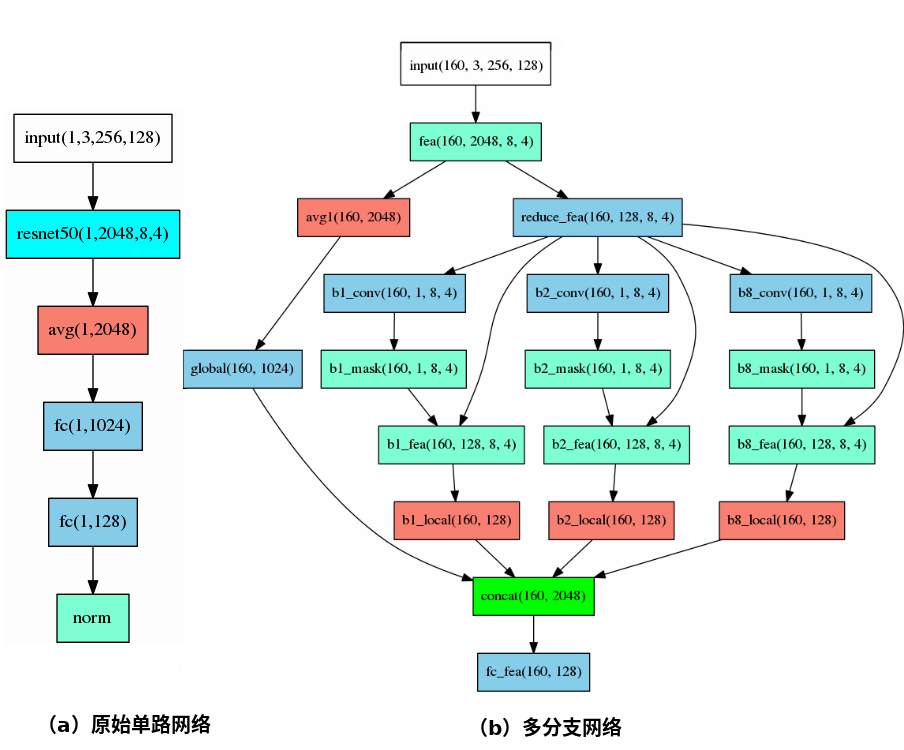
\includegraphics[width=.95\textwidth]{branch.png} 
% 	\caption{多分支模型}
% \end{figure}

\subsection{特征融合与度量学习模块}

在特征融合方式上,我们尝试了很多种模式,包括
\textbf{(1)、}先将中层特征和全局特种嵌入到共享的128维空间,然后自适应求和得到紧凑的特征表示;
\textbf{(2)、}直接将各个层次的特征拼接,引入Dropout机制防止过拟合,通过全连接层的权重自适应地获得128维空间的嵌入表示;
\textbf{(3)、}使用特征本身作为输入求得权重对特征进行变换。这种方法的特性是注意力权重由输入动态决定,但是由于在从特征到权重的过程中不可避免地要学习全连接层权重,这种方式在一定程度上退化为了第二种方法。

通过实验,我们最终采用了图~\ref{fig:fusion}的特征融合方式。首先对中层特征进行通道层面的属性特征注意力重组,全局池化抽取中层属性特征,然后与最后的语义表示通过拼接的方式形成最终的特征表示。值得注意的是,在基于注意力机制重新组合特征的过程中,我们已经获得了这一阶段的属性表示。
重用该属性表示,我们既没有引入过多的计算,
又有助于深层监督信息更加容易地反传监督中层属性特征的学习。

\begin{figure}
	\centering
	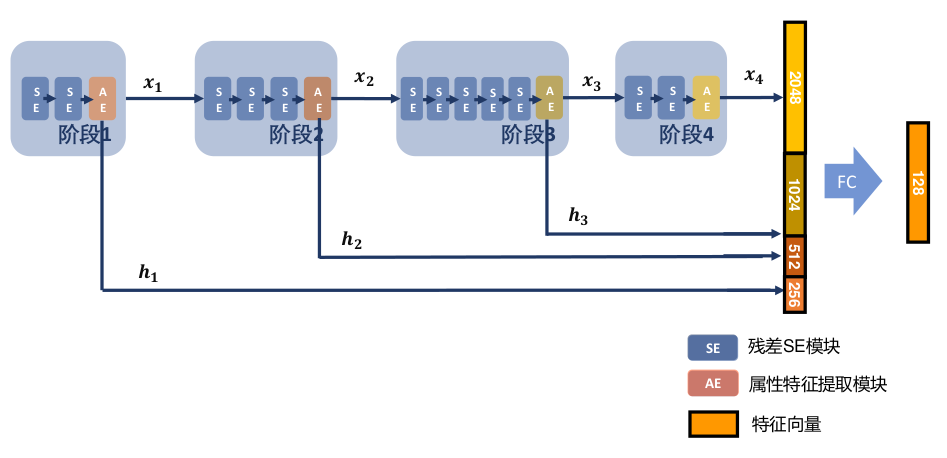
\includegraphics[width=.9\textwidth]{fig/2018-05-11-16-54-07.png}
	\caption{中层特征与全局特征的融合方式}
	\label{fig:fusion}
\end{figure}

由于我们的目标是直接学习128维度的嵌入特征,因此我们采用了更为合适的度量学习方法---基于难样本挖掘的三元组损失\cite{hermans2017defense}。
在损失计算的过称中,我们会选择从随机生成的批样本中最难的样本对$(\mX_a, \mX_p, \mX_n)$,
其中 $(\mX_p, \mX_a)$是属于同一行人的正样本对
, $(\mX_n, \mX_a)$是属于不同行人的负样本对。
我们采用 $\vx_a, \vx_p, \vx_n$表示每个样本经过深度网络获得的
嵌入表示。则基于难样本挖掘的三元组损失如公式~\ref{eq:trihard}所示。
\begin{equation}
	\cL_{\textrm{TriHard}} (\mX, \vtheta) = \sum_{a=1}^{N} \max\left(
	0, m + \min_{\substack{
			p=1...N \\
			y_a = y_p}
	} D(\vx_a, \vx_p)
	-  \max_{ \substack{
			n=1...N \\
			y_a \neq y_n }
	} D(\vx_a,\vx_n)
	\right) \label{eq:trihard}
\end{equation}

其中,难样本体现在求最远的正样本和最近的负样本上。锚点样本会循环遍历整个小批次样本集合(mini-batch),
找到对应的 $\vx_p$嵌入空间中最远最难的正样本和 $\vx_n$ 最近最难的负样本,计算单个样本的损失函数。

\section{实验设计和结果}

\subsection{数据集信息与评估协议}

% copy ...
我们提出的算法在六个广泛使用的数据集里训练和评测,这六个数据集分别是CUHK03 \cite{li2014deepreid}, Market1501 \cite{zheng2015scalable},  CUHK01 \cite{li2013locally}, DukeMTMC \cite{zheng2017unlabeled}, \cite{ristani2016MTMC} , and VIPeR \cite{gray2007evaluating}。
表~\ref{table:dataset}列出了各个数据集的统计信息和普遍遵循的训练测试划分协议。

% \begin{itemize}
% 	\item
\textbf{CUHK01数据集}包含两个摄像头拍摄到的971 个行人,3884 张行人图像,平均每个行人包含来自不同摄像头的图片各两张。两个摄像头之间存在近乎90度的视角变化,因此难度较大。普遍遵循的训练测试划分协议有100 个测试身份和485个测试身份两种版本。为了方便和文献中方法进行比较,我们在两种协议下都做了相应的实验。
% \item

\textbf{CUHK03数据集}对CUHK01数据集进行了大幅扩充,包含1360个行人,13164张行人图像。它的评估协议有两个版本,
	分别是人工标注行人边框形成的数据集
	和DPM行人检测器自动生成边框的数据集
	。
对于检测器自动生成的数据集,平均每个行人拥有10 张图像,平均每个监控视角5张。对于人工标注的数据集,平均每个监控视角每个行人有4.7张图像。
	同样为了方便比较,
	我们在两个版本的数据集上都做了实验。
	% todo cuhk03 new protocol 
% \item

\textbf{ViPeR数据集}是一个较小的数据集,
	它包含
	来自两个视角无重叠的623个行人目标。
	每个行人在
	在单个视角里每个行人仅有一张图像。
% \item

\textbf{PRID450s数据集}共包含450个行人的900张图片。每个行人都有来自两个室外摄像头的一对图像,摄像头之间的光照、视角、相机参数的差异增加了该数据集的难度。
% \item

\textbf{i-LIDS数据集}由在机场到达大厅收集的视频监控构建的,存在一定的行李遮挡情况。它包含119个行人的479张图像,平均每个行人有4张图片。
% \item

\textbf{PRID2011数据集}包含从两个固定摄像头里捕捉到行人图像,虽然两个视角各有385和749个行人图像,但是两个摄像头共有的行人只有200个。遵循以往工作,我们采用100个身份作为训练集,剩下个100个作为测试机。
	在测试时,使用一个视角下的100张图像作为查询图像,另一个视角下的100张相同身份的行人图像和剩下所有图像作为搜索库。
% \end{itemize}

为了衡量我们提出的基于多尺度特征融合方法的性能,
我们采用累积匹配因子(Cumulative Matching Characteristics,CMC)指标和mAP指标。CMC指标衡量了从样本库里找到的样本正确排在查询列表前面的频次;
mAP指标综合衡量了整个预测列表与预期结果之间的差距。
% todo cmc-1 all protocol mAP

\begin{table}
	\centering
	\caption{数据集统计信息和训练测试划分协议}
	\label{table:dataset}
	\begin{tabular}{llllll}
		\toprule
		Dataset    & CUHK03 & Market1501 & CUHK01  & DukeMTMC & VIPeR \\
		\midrule
		identities & 1,467  & 1,501      & 971     & 1,812    & 632   \\
		images     & 13,164 & 32,668     & 3,884   & 36,411   & 1,264 \\
		views      & 2      & 6          & 2       & 8        & 2     \\
		train IDs  & 1,367  & 751        & 871/485 & 702      & 316   \\
		test IDs   & 100    & 751        & 100/486 & 1110     & 316   \\
		\bottomrule
	\end{tabular}
\end{table}

\subsection{实验结果和比较}

\begin{table}
	\centering
	\caption{在数据集CUHK03上的CMC-1,CMC-5,CMC-10性能指标比对}
	% \scalebox{0.95}{
	\begin{tabular}{c|ccc|ccc}
		\hline
		\multirow{2}*{Methods}               &
		\multicolumn{3}{c|}{labelled CUHK03} &
		\multicolumn{3}{c}{detected CUHK03}                                                                                                        \\
		\cline{2-7}
		\cline{2-7}
		                                     & r=1            & r=5            & r=10           & r=1            & r=5            & r=10           \\ \midrule
		KISSME                               & 14.17          & 37.46          & 52.20          & 11.70          & 33.45          & 45.69          \\
		LMNN                                 & 7.29           & 19.64          & 30.74          & 6.25           & 17.87          & 26.60          \\
		LOMO+XQDA                            & 52.20          & 82.23          & 92.14          & 46.25          & 78.90          & 88.55          \\ \hline
		ImprovedDL                           & 54.74          & 86.50          & 93.88          & 44.96          & 76.01          & 81.85          \\
		DCSL (with hnm)                      & 80.20          & 97.73          & 99.17          & -              & -              & -              \\
		JLML                                 & 83.20          & 98.00          & 99.40          & 80.60          & \textbf{96.90} & \textbf{98.70} \\ \hline
		SC-PPMN (with hnm)                   & \textbf{85.50} & \textbf{98.20} & \textbf{99.50} & \textbf{80.63} & 95.62          & 98.07          \\ \hline
		\hline
		TriHard Baseline                     &84.91 86.28  & 98.11 &  99.27            & 82.79          &                &                \\
		+ SE Attention                       & 84.79 88.28 & 98.50 &  99.24              & 85.50          &                &                \\
		+ Multi-Scale Fusion                 &  85.66  88.28 & 98.44 &  99.24               & 85.93          &                &                \\
		+ Rerank                             & 96.34     96.34     &                &                & 91.53          &                &                \\
		\hline
	\end{tabular}
	\label{tab:cuhk03}
\end{table}



\begin{table}
	\centering
	\caption{在数据集Market1501上的CMC-1,CMC-5,mAP性能指标对比}
	\label{tab:market}
	\begin{tabular}{c|ccc|ccc}
		\toprule
		\multirow{2}*{Methods}          &
		\multicolumn{3}{c|}{Market1501} &
		\multicolumn{3}{c}{DukeMTMC}                                            \\
		\cline{2-7}
		\cline{2-7}
		                                & r=1   & r=5 & mAP   & r=1 & r=5 & mAP \\ \midrule
		TriHard Baseline                & 85.61 &     & 69.53 &     &     &     \\
		+ SE Attention                  & 87.47 &     & 72.27 &     &     &     \\
		+ Multi-Scale Fusion            & 88.53 &     & 72.86 &     &     &     \\
		+ Rerank                        & 89.40 &     &       &     &     &     \\
	\end{tabular}
\end{table}


\begin{table}[htbp]
	\centering
	\caption{在数据集CUHK01上的性能比对。表中列出了CMC(\%)指标在rank-1,rank-5和 rank-10 的结果。}
	% \scalebox{0.95}{
	\begin{tabular}{c|ccc|ccc}
		\hline
		\multirow{2}*{Methods}                    & 
		\multicolumn{3}{c|}{CUHK01(100 test IDs)} & 
		\multicolumn{3}{c}{CUHK01(486 test IDs)}                                                                                                        \\
		\cline{2-7}
		                                          & r=1            & r=5            & r=10           & r=1            & r=5            & r=10           \\ \hline
		KISSME                                    & 29.40          & 60.18          & 74.44          & -              & -              & -              \\
		LMNN                                      & 21.17          & 48.51          & 62.98          & 13.45          & 31.33          & 42.25          \\
		LSSCDL                                    & 65.97          & 48.51          & 62.98          & -              & -              & -              \\ \hline
		\hline
		FPNN                                      & 27.87          & 59.64          & 73.53          & -              & -              & -              \\
		ImprovedDL                                & 65.00          & 89.00          & 94.00          & 47.53          & 71.60          & 80.25          \\
		SICIR                                     & 71.80          & -              & -              & -              & -              & -              \\
		TCP                                       & -              & -              & -              & 53.70          & 84.30          & 91.00          \\
		MTDnet-cross                              & 78.50          & 96.50          & 97.50          & -              & -              & -              \\
		DCSL (no hnm)                             & 88.00          & 96.90          & 98.10          & -              & -              & -              \\
		DCSL (hnm)                                & 89.60          & 97.80          & 98.90          & 76.54          & 94.24          & 97.49          \\ \hline
		SC-PPMN (no hnm)                          & 92.10          & 99.50          & 99.95          & -              & -              & -              \\
		SC-PPMN (hnm)                             & \textbf{93.10} & \textbf{98.80} & \textbf{99.80} & \textbf{77.16} & \textbf{92.80} & \textbf{97.53} \\ \hline
		\bottomrule
	\end{tabular}
	
	\label{table:CUHK01}
\end{table}

\begin{table}[htbp]
	\centering
	\caption{在数据集VIPeR和PRID450s上的CMC-1,CMC-5,CMC-10性能指标比对}
	%\scalebox{0.95}{
	\begin{tabular}{c|ccc|ccc}
		\hline
		\multirow{2}*{Methods}     &
		\multicolumn{3}{c|}{VIPeR} &
		\multicolumn{3}{c}{PRID450s}                                                                                            \\
		\cline{2-7}
		                           & r=1            & r=5            & r=10           & r=1            & r=5   & r=10           \\ \hline
		KISSME                     & 19.60          & 48.00          & 62.20          & 15.0           & -     & 39.0           \\
		LSSCDL                     & 42.66          & -              & 84.27          & 60.49          & -     & 88.58          \\
		LOMO+LSTM                  & 42.40          & 68.70          & 79.40          & -              & -     & -              \\
		LOMO+XQDA                  & 40.00          & 68.13          & 80.51          & \textbf{61.42} & -     & \textbf{90.84} \\ \hline
		\hline
		ImprovedDL                 & 34.81          & 63.61          & 75.63          & 34.81          & 63.72 & 76.24          \\
		PIE(R)                     & 27.44          & 43.01          & 50.82          & -              & -     & -              \\
		SICIR                      & 35.76          & -              & -              & -              & -     & -              \\
		TCP                        & 47.80          & 74.70          & 84.80          & -              & -     & -              \\
		DCSL                       & 44.62          & 73.42          & 82.59          & -              & -     & -              \\
		JLML                       & \textbf{50.20} & 74.20          & 84.30          & -              & -     & -              \\ \hline
		SC-PPMN                    & 45.82          & \textbf{74.68} & \textbf{86.08} & 52.08          & 82.58 & 88.36          \\ \hline
		TriHard Baseline            &          &                &                &           &                &                \\
		+ SE Attention              &            &                &                &          &                &                \\
		+ Multi-Scale Fusion        &          &                &                &          &                &                \\
		+ Rerank                    &           &                &                &           &                &                \\
	\end{tabular}
	%}

	\label{table:viper}
	% \vspace{-1ex}
\end{table}

\begin{table}[htbp]
	\centering
	\caption{在数据集i-LIDS和PRID2011上的CMC-1,CMC-5,CMC-10性能指标比对}
	%\scalebox{0.95}{
	\begin{tabular}{c|ccc|ccc}
		\hline
		\multirow{2}*{Methods}      &
		\multicolumn{3}{c|}{i-LIDS} &
		\multicolumn{3}{c}{PRID2011}                                                                                                      \\
		\cline{2-7}
		                            & r=1            & r=5            & r=10           & r=1            & r=5            & r=10           \\ \hline
		ITML                        & 29.00          & 54.00          & 70.50          & 12.00          & -              & 36.00          \\
		KISSME                      & -              & -              & -              & 15.00          & -              & 39.00          \\
		LMNN                        & 28.00          & 53.80          & 66.10          & 10.00          & -              & 30.00          \\ \hline
		\hline
		TCP                         & \textbf{60.40} & \textbf{82.70} & 90.70          & 22.00          & 47.00          & 57.00          \\
		MTDnet                      & 57.8           & 78.61          & 87.28          & \textbf{32.00} & 51.00          & 62.00          \\
		\hline
		SC-PPMN                     & 54.80          & 81.92          & \textbf{92.32} & \textbf{32.00} & \textbf{53.00} & \textbf{63.00} \\ \hline
		TriHard Baseline            &          &                &                &           &                &                \\
		+ SE Attention              &            &                &                &          &                &                \\
		+ Multi-Scale Fusion        &          &                &                &          &                &                \\
		+ Rerank                    &           &                &                &           &                &                \\
	\end{tabular}
	%}

	\label{table:ilids}
\end{table}


\section{本章小结}

% -------------------------------------------------------------------------
\chapter{基于对比中心损失的度量学习}
% -------------------------------------------------------------------------

\section{问题描述}

行人再识别问题是图像检索的子问题,它的输入通常是一些从未在训练集中出现过的行人图片,我们最终希望获得的是能广泛应用于各种情况下行人图像对的距离度量函数。
因此度量学习更加适用于行人再识别。

在早期的文献中,度量学习的目标是学习一个相似性函数。通常采用马氏距离
$\norm{\vx_1 - \vx_2}_\mM=
	\sqrt{(\vx_1-\vx_2)^T \mM (\vx_1 - \vx_2) }$
作为相似性度量,学习其中的半正定矩阵$\mM$。
但是在最近的文献中,往往使用神经网络自动学习深度嵌入特征$\vx_1, \vx_2$,而使用最简单的距离度量---欧式距离。
通过在欧式空间中设计
带有间隔(margin)损失函数
直接学习行人图片在欧式度量嵌入空间中的
特征表示。
因此,从某种程度上来说,现有的度量学习已经转化为了特征学习的过程。
典型的损失函数包括对比损失、三元组损失,
他们都在特征空间中定义了直观的损失函数,使用欧氏距离作为特征空间的度量函数,深度网络作为核函数,端到端地学习图像空间的非线性度量函数。

从是否给每个类别创建模板的角度,损失函数可以分为基于模板的损失和基于实例的损失。
从度量函数的角度,损失函数可以分为基于交叉熵的损失和基于欧式间隔的损失。(虽然交叉熵严格来说不属于度量函数,因为它不具有对称性。但它却是广泛用于表征两个概率分布之间的距离。)
% 比如Zheng?使用Logistic损失函数对“同一行人的类内距离小于不同行人的类间距离”这一事件的概率建模,得到了PRDC模型。
% 图是怎么来的。。。

我们首先在大型数据集上可视化分析各个损失的优缺点,然后基于我们的观察提取对比中心损失。值得一提的是我们提出的损失函数与先有的最新工作能够相互适应、相互提升。比如进一步引入上一节中注意力机制\misscite,或最新的网络结构\misscite, 我们的方法仍能获得进一步的提升。

\section{研究方法}
\subsection{损失函数分类与优缺点分析}
每一种损失都有各自的优缺点,如图~\ref{fig:losses}所示,这是在CUHK03数据集上选取50个类别和全部样本可视化,红色三角形代表类别中心,蓝色和黄色圆形代表每一类别的实例。
\textbf{(a)、}中心损失虽然成功学到了每个类别的中心,
但是对各个类别给以相同的重视程度,而忽略了
每个类别区分难易度不同的事实,
因此部分类心很容易与临近的类心混淆;
另一方面,存在一些标注错误或实在困难的样本,容易和临近类心混淆。
对于这样的样本,与其使用相同的权重,使得它尽可能接近类心,倒不如忽视这样的样本,防止过拟合,以便获得一个对大部分样本泛化能力好的特征提取器。
\textbf{(b)、}
传统的基于模板的损失具有较高的计算效率,因为它会为每个类别创建学习模板,而这样的模板包含了整个数据集中某一类别的所有信息,并且随着深度网络的训练不断被迭代更新。
在ImageNet大规模分类时代做出了重大贡献。但是对于再识别问题,它有一定的缺点。
如图~\ref{fig:losses}所示,交叉损失的分类器权重被视为类心向量与样本特征向量共同嵌入到2维空间可视化,
显然在训练集上每个特征向量被成功聚拢在了对应类别中心定义的区域内部;
在测试集上特征向量虽然也成功被分为了不同的类别,但是却很容易与相邻类别混淆。
% todo 测试集
这就是所说的具有可分性,但是不具有鉴别性。
这样的特征向量只能用于封闭环境的分类问题,无法适应开放环境的再识别问题。
\textbf{(c)、}
三元组损失关注样本对之间的细粒度的关系,有时候会比样本与模板之间的关系包含更多信息。
基于难样本挖掘的三元损失成功挖掘了这样的信息,
为不同的类别拉开了一定的距离,但是仍然具有较大的类内散度。

\begin{figure}
	\centering
	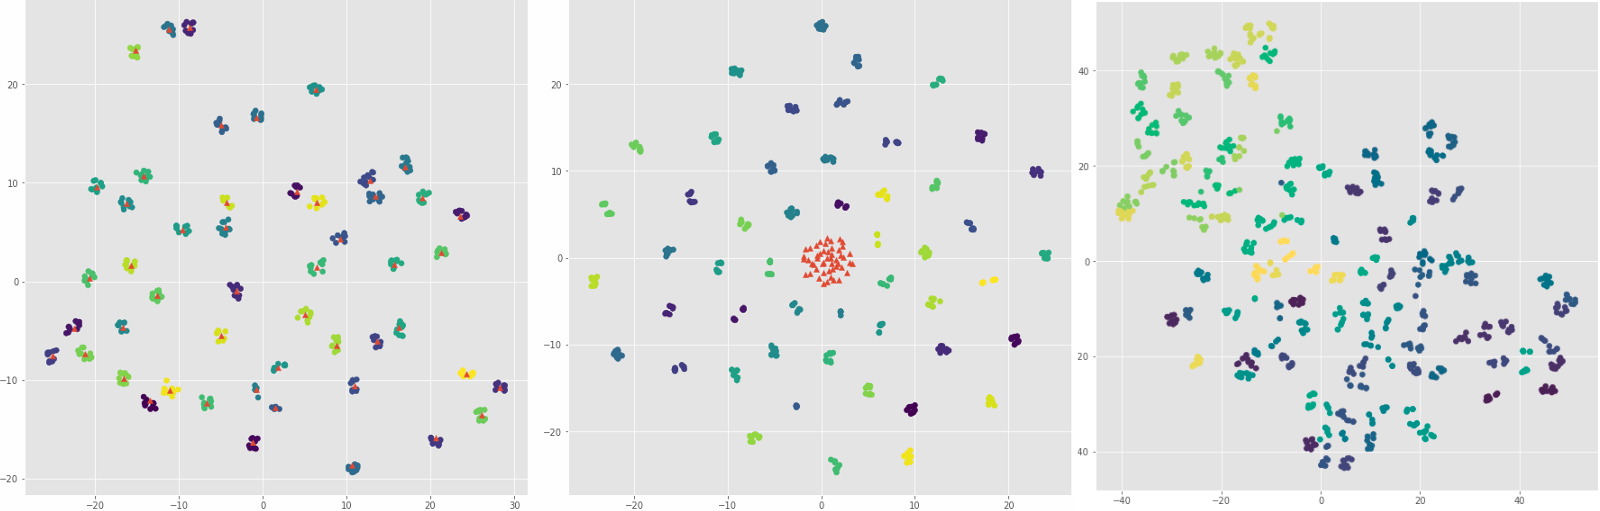
\includegraphics[width=.95\textwidth]{losses.png}
	\caption{三种损失函数监督的验证集特征向量和中心向量在2维平面上降维可视化,使用CUHK03数据集和各损失的基准模型得到}
	\label{fig:losses}
\end{figure}

基于难样本挖掘的三元组损失的缺点可以进一步在图~\ref{fig:tsne}中观察到,尽管验证集上的类内散度已经很小了,
但是由于在测试集上存在一些样本偏离到边界,
容易和临近的类别混淆。
就是这样的一些样本造成了性能指标的下降。

\begin{figure}
	\centering
	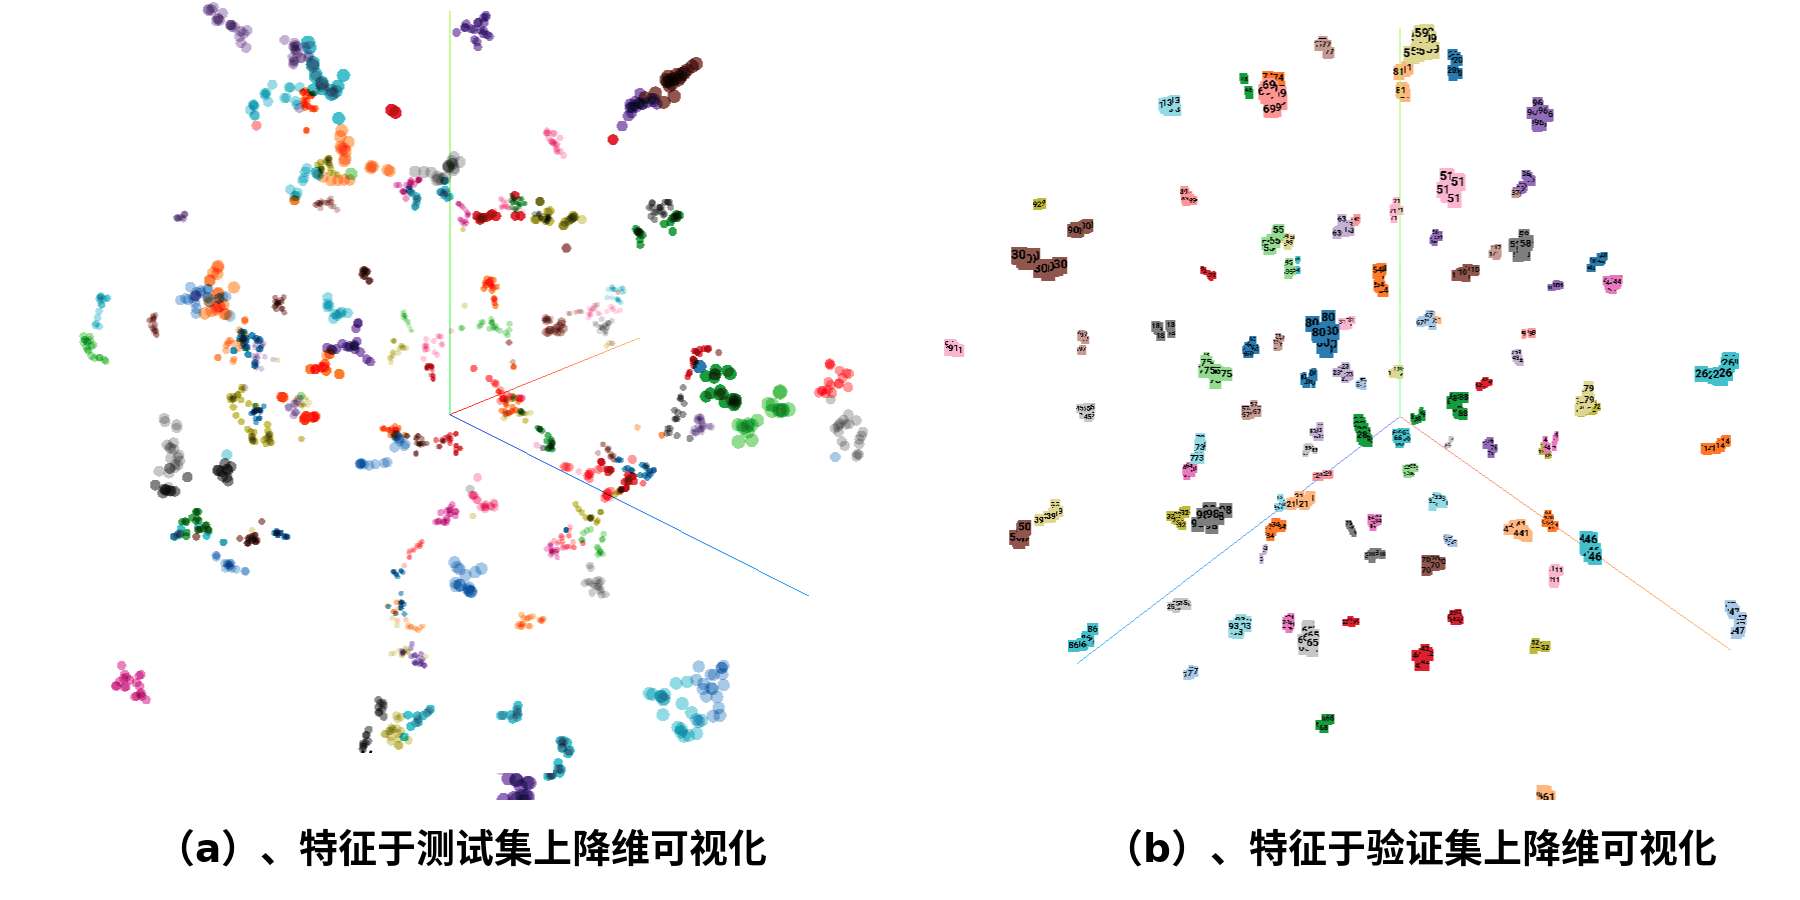
\includegraphics[width=.95\textwidth]{tsne.png}
	\caption{三元组损失在3维空间降维可视化,使用CUHK03数据集和我们的基准模型得到}
	\label{fig:tsne}
\end{figure}

\subsection{对比中心损失}

首先对我们所采用的符号进行说明。
假设训练集可以表示为,$\cT=\{(\mX_i,y_i)\}_{i=1}^{N^{\textrm{train}}}$, 由$N^{\textrm{train}}$个图片样本
$\mX_i \in \real^{W\times H\times C}$
% with $\vx_i \in \real^{F}$ 
和M各类别的
标签$y_i \in \{1,\dots, M\}$组成。
最近一些文献中度量学习的目标可以总结为
学习一个特征提取函数
$\vx = \vf_\vtheta (\mX): \real^{W \times H\times C} \rightarrow \Rbb^D$,
将语义上相似的点从数据流形上映射到特定度量(通常是欧氏度量)下相近的点。
一般形式的特定度量可以表示为$D( \vx_i, \vx_j):\Rbb^D \times \Rbb^D \rightarrow \Rbb$,
通常采用的欧式度量为
$D(\vx_i,\vx_j)=\|\vx_i - \vx_j\|_2$。
如果特征空间中的度量函数采用
$D(\vx_i,  \vx_j)$的形式,那么在图像空间中的度量函数可以表示为
$D(\vf_\vtheta(\mX_i), \vf_\vtheta(\mX_j))$。
在后续的叙述中,为了简化公式我们会采用$D(\vx_i,  \vx_j)$的形式,看起来它是没有参数的,
但是事实上$\vx$ 是被 $\vtheta$参数化的,也即损失会通过欧式度量反向传播更新特征提取网络的参数。
类是地,
为了简化公式,我们会采用
$D(\vx_i,\vc_j)$表示样本和中心在特征空间的距离
,而不是$D(\vf_\vtheta(\mX_i), \vc_j)$.

与上一节\misscite 相同,我们仍然采用基于难样本挖掘的三元组损失作为基准模型。其公式参见\misscite 。在实践中,我们观察到
% TODO , , 
在训练后期,这类基于实例的损失还是不可避免地会饱和,并且出现大量零梯度。这是因为尽管使用了批样本内部的挖掘,但是形成批样本的过程仍然是随机的。于是,有可能出现的情况是:在训练后期,形成的一整个批样本都不包含有效三元组,即所有三元组都已经满足 
\misscite  
所定义的间隔要求。而这个现象在CUHK03数据集上尤为突出,因为这个行人再识别数据集包含很多不同的行人,同时每个行人的训练正样本只有不到10张(平均9所定义的间隔要求。而这个现象在CUHK03数据集上尤为突出,因为这个行人再识别数据集包含很多不同的行人,同时每个行人的训练正样本只有不到10张(平均9.4张)。基于这个观察,我们结合基于模板的损失,在形成批样本的时候引入难类别挖掘,消除基于实例的损失训练饱和的问题。

我们首先尝试中心损失,这种损失直接基于欧式度量学习每个类别的中心$\vc_{y_i}$,并将对应类别的样本$\vx_i$拉向中心$\vc_{y_i}$。
\begin{equation}
	\cL_{\textrm{Cent}} (\mX, \mC, \vtheta) = \frac{1}{2}
	\sum_{i=1}^{N}  D(
	\vx_i , \vc_{y_i} )
\end{equation}

但是这种损失仍然面临着正样本不足,没有足够的统计信息更新中心模板的问题。
同时这种损失隐式地给每个样本-中心对赋予了相同的权重,显然不符合真实世界的数据分布。
于是我们提出了对比中心损失,
\begin{equation}
	\cL_{\textrm{CCent}} (\mX, \mC, \vtheta) = \frac{1}{2}
	\sum_{i=1}^{N}
	\frac{D(
		\vx_{i}, \vc_{y_i}
		)}{ 
			\displaystyle w_s
			\min_{\substack{
				j=1...M \\
				j \neq y_i }}
		D(
		\vx_{i}, \vc_{j}
		) + 1 }
	-
	\lambda_d \sum_{i=1}^{M}  \min_{j=1...M} D(\vc_i,\vc_j)
\end{equation}

式子中涉及到两个超参数$w_s$和$\lambda$。

$w_s$用于对样本和正类中心之间的距离进行缩放,$\min_{\substack{
				j=1...M \\
				j \neq y_i }} D(
		\vx_{i}, \vc_{j}
		)$
会进一步根据样本到最近的负类中心的距离进行缩放。
对比的思想样本到正类中心距离和样本到负类中心距离相除的过程中。
从前向的角度看,多考虑一个负类中心的好处在于根据数据分布本身的特性,动态地给不同的样本-中心对以不同的权重。同时有助于将损失归一化到一定的范围内。
从反向传播的角度看,多考虑一个负类能提高样本的利用效率。使用一个样本同时更新了正类和最难的负类,能加快类别中心的学习进程。
考虑到大多数的再识别任务中,类别数目可以达到1k,甚至4k。我们只选取最难的负类来减少反向传播时候的计算量。
事实上,在大多时候,一个样本只会被误判为少数几个身份,因此选取最难的负类中心,已经提供了绝大部分信息。
当$w_s$趋近于0时候,中心对比损失退化为中心损失;当$w_s$趋近于1时,中心对比损失表现地和交叉熵损失较为类似。

$\lambda_d$用于权衡类内散度和类间散度。为了避免相同的类别中心对不断地被优化(这样的类别中心往往是由于标注错误产生的异常类别),
我们使用所有类别中心对中距离最小的$\min_{j=1...M} D(\vc_i,\vc_j)$进行优化。
这是所有可能类别中心对中最容易被混淆的一对。
由于随机选取批梯度(每次会有不同类别的样本进入批样本),
加上每次只取最容易被混淆的一对优化,我们可以有效避免深度网络过度强调特定的类别中心对。
这一项可以看作对类心权重模板的正则化,
使得类心模板尽可能均匀地散布在特征空间。


\section{结果验证和分析}

% -------------------------------------------------------------------------
\chapter{结论与展望}
% -------------------------------------------------------------------------

\section{结论}



\section{展望}

在实验中,我们发现了很多其他有意思的现象。比如,\misscite 提出在人脸识别中使用$L_2$归一化的特征向量,
有助于稳定深度网络,并提升性能。但是在实验中,我发现稳定深度网络的关键因素是对维度变换前的2048维向量进行批归一化(BatchNormalize),
至于是否对最终的128维特征使用$L_2$归一化,
无论是对是否收敛、还是收敛后的性能,都没有绝对的影响。





% \bibliographystyle{assets/gbt7714-2005}
% {
\printbibliography[heading=chapbib]
% }
